\section{Dados Especialistas}
Para facilitar a inserção de dados especialistas foi criado uma \textit{interface} para mapear possíveis questões da EADS nos tweets. Para ativar a plataforma de inserção de dados especialistas basta utilizar o comando \textit{docker-compose up specialist\_app}, caso deseje subir essa aplicação online será necessário um serviço de núvem, porém, a aplicação rodada local pode ser acessada para \textit{\url{http://localhost:3000}}.

Os dados foram inseridos manualmente simulando especialistas, sem lógica de ponderação. Todos os dados que serão apresentados foram anotados pelo autor e não por especialistas. A partir disso foram encontrados na análise 312 tweets com perguntas inseridas, entretanto, um tweet pode responder mais de uma pergunta, foram inseridas um total de 688 perguntas. Como apresentado na Figura \ref{fig:question-balance} e conforme o Anexo \ref{app:eads} é possível ver que as questões que mais contém respostas são questões mais voltadas a situação psicológica, sendo mais frequente expressá-las involuntáriamente durante seu discurso. Em contra partida as perguntas com menos respostas, são as questões referentes a situações fisicas.

\begin{figure}[!ht]
    \centering
    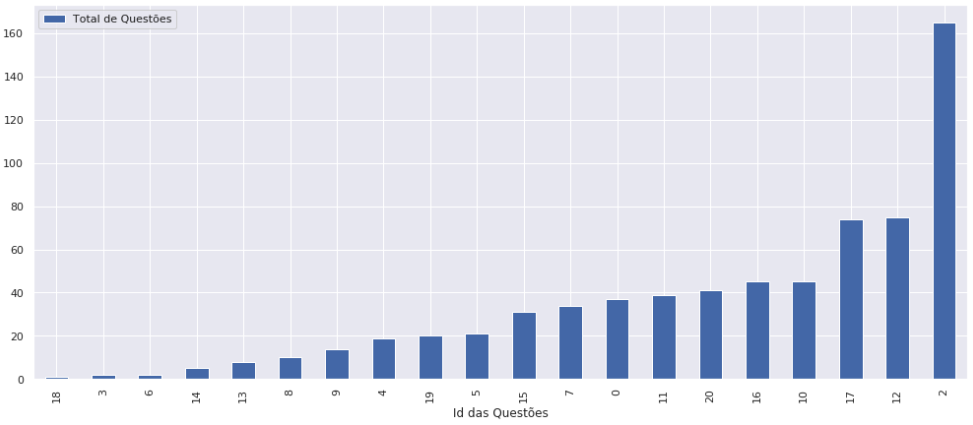
\includegraphics[width=.75\textwidth]{imagens/question-balance.png}
    \caption{Relação de Perguntas Respondidas por Tweets}
    \label{fig:question-balance}
\end{figure}

As questões com menor resposta estão atreladas com ansiedade conforme Anexo \ref{app:eads}, isso afeta o desempenho do projeto final, entretanto, é possível encontrar relações e aproximar os valores para chegar no resultado final. Em primeiro momento o objetivo é apenas inferir perguntas (ignorando até mesmo o impacto), já que não existem informações suficientes relacionadas a essas questões a máquina não conseguira inferir essa informação, entretanto, não irá impedir que as demais perguntas sejam devidamente inferidas.

